\section{Durchführung}
\label{sec:Durchführung}
Um die effektive Masse der Leitungselektronen in n-dotierten Galliumarsenid zu bestimmen, werden in diesem Versuch zwei dotierte Proben mit unterschiedlicher 
Donatorenkonzentration und eine undotierte GaAs Probe analysiert. Dazu wird die Faradayrotation eines Lichtstrahls nach dem Durchqueren der Proben für 
verschiedene Wellenlängen ermittelt. Aus der Proportionalität des Drehwinkels zum Quadrat der Wellenlänge lässt sich sodann die effektive Masse der Elektronen
errechnen.

\subsection{Versuchsaufbau}
\label{subsec:Versuchsaufbau}
Um den Drehwinkel der Faradayrotation zu ermitteln wird der in \autoref{fig:Aufbau} gezeigte Aufbau verwendet.
\begin{figure}
    \centering
    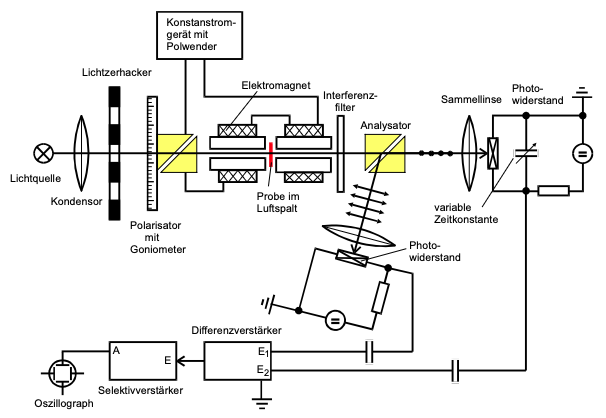
\includegraphics[width=.8\textwidth]{content/pics/Aufbau.png}
    \caption{Skizze des verwendeten Versuchsaufbaus zur Messung der Faradayrotation mithilfe des Zweistrahlverfahrens \cite{V46}.}
    \label{fig:Aufbau}
\end{figure}
Als Lichtquelle wird eine Halogenlampe verwendet, die Licht im sichtbaren- und Infrarotbereich aussendet. Die zu analysierende Wellenlänge kann mittels 
Interferenzfiltern separiert werden. Nach der Fokussierung des Strahles durchläuft dieser ein \textit{Glan-Thompson-Prisma}, welches das emmitierte Licht 
linear polarisiert. Dieser Polarisator ist um die Strahlachse drehbar gelagert und mit einem Goniometer versehen, anhand dessen sich der Drehwinkel des Prismas 
genau ablesen lässt. Die Probe wird in der Mitte eines Elektromagneten platziert, dessen Magnetfeld über ein Konstantstromgerät eingestellt werden kann. 
Hinter dem Elektromagneten befindet sich eine Haltevorrichtung für die zuvor erwähnten Interferenzfilter und ein weiteres Glan-Thompson-Prisma. Dieses dient als 
Analysator und teilt den eintreffenden Strahl in zwei genau senkrecht zueinander polarisierte Teilstrahlen auf. Die Intensität der beiden Teilstrahlen kann anschließend 
über zwei Photowiderstände gemessen werden. Über einen Differenzverstärker kann die Differenz der Signale der beiden Teilstrahlen an einem 
Oszilloskop dargestellt werden. Wie in \autoref{fig:Aufbau} zu erkennen ist, sind außerdem ein \glqq Lichtzerhacker\grqq{} und ein Selektivverstärker verbaut. 
Mit Hilfe des Lichtzerhackers wird der Lichtstrahl in Einzelbündel mit einer Frequenz von $\qty{450}{\hertz}$ unterteilt. Der Selektivverstärker wird auf dieselbe 
Frequenz eingestellt, was zur Unterdrückung von Rauschspannungen in anderen Frequenzbereichen dient.

\subsection{Justierung der Messapparatur}
Vor Beginn der eigentlichen Messung muss die Messapparatur justiert werden. Dazu wird zuerst die korrekte Installation der optischen Elemente überprüft. 
So sollte sich die gemessene Spannung an jeweils einer der beiden Photowiderstände durch Rotation des Polarisator-Prismas mit einer Periodizität von $\qty{90}{\degree}$ 
auf Null regeln lassen. Des Weiteren sollte überprüft werden, ob die Teilstrahlen auf die lichtempfindlichen Flächen der Photowiderstände abgebildet werden. 
Sind alle optischen Elemente justiert, wird der Selektivverstärker auf die Frequenz des Lichtzerhackers abgestimmt. Dazu wird die Frequenz des Selektivverstärker 
im Bereich der am Lichtzerhacker eingestellten Frequenz variiert. Es wird die Frequenz eingestellt, bei der die Amplitude des Signals der Photowiderstände maximal ist.
Nun kann mit der eigentlichen Messung begonnen werden.

\subsection{Messung der Faradayrotation}
\label{subsec:Messung der Faradayrotation}
Zur Messung des Drehwinkels der Faradayrotation werden neun verschiedene Interferenzfilter mit Wellenlängenbereichen von $\num{1.06}$ bis $\qty{2.65}{\micro\metre}$ verwendet.
Nach dem Einsetzen einer Probe und eines Interferenzfilters wird mithilfe des drehbaren Polarisators ein Winkel $\theta_1$ eingestellt, der die Amplitude des Signals des 
Differenzverstärkers 
minimiert. Anschließend wird die Polung des Elektromagneten umgestellt, sodass ein genau entgegengerichtetes Magnetfeld entsteht. Erneut wird die Amplitude minimiert und der 
zugehörige Winkel $\theta_2$ notiert. Da mit dieser Methode das Magnetfeld um $2B$ geändert wird, berechnet sich der Drehwinkel der Faradayrotation zu 
\begin{equation}
    \label{eqn:theta_diff}
    \theta = \frac{1}{2}(\theta_1 -\theta_2).
\end{equation}

\subsection{Messung des \textbf{B}-Felds}
\label{subsec:Messung des B-Felds}
Zur Bestimmung der effektiven Elektronenmasse muss die magnetische Flussdichte $B$ im Bereich der Probe bekannt sein. Mit einer auf einem Stativ befestigten Hallsonde 
wird die Flussdichte des Magnetfeldes entlang der Strahlachse vermessen. Es werden Messwerte im Abstand von wenigen Millimetern um den Probenbereich genommen. 
Das Maximum der Messreihe wird in der Rechnung zur Bestimmung der effektiven Elektronenmasse verwendet.
